\documentclass[12pt]{article}\usepackage[]{graphicx}\usepackage[]{color}
%% maxwidth is the original width if it is less than linewidth
%% otherwise use linewidth (to make sure the graphics do not exceed the margin)
\makeatletter
\def\maxwidth{ %
  \ifdim\Gin@nat@width>\linewidth
    \linewidth
  \else
    \Gin@nat@width
  \fi
}
\makeatother

\definecolor{fgcolor}{rgb}{0.345, 0.345, 0.345}
\newcommand{\hlnum}[1]{\textcolor[rgb]{0.686,0.059,0.569}{#1}}%
\newcommand{\hlstr}[1]{\textcolor[rgb]{0.192,0.494,0.8}{#1}}%
\newcommand{\hlcom}[1]{\textcolor[rgb]{0.678,0.584,0.686}{\textit{#1}}}%
\newcommand{\hlopt}[1]{\textcolor[rgb]{0,0,0}{#1}}%
\newcommand{\hlstd}[1]{\textcolor[rgb]{0.345,0.345,0.345}{#1}}%
\newcommand{\hlkwa}[1]{\textcolor[rgb]{0.161,0.373,0.58}{\textbf{#1}}}%
\newcommand{\hlkwb}[1]{\textcolor[rgb]{0.69,0.353,0.396}{#1}}%
\newcommand{\hlkwc}[1]{\textcolor[rgb]{0.333,0.667,0.333}{#1}}%
\newcommand{\hlkwd}[1]{\textcolor[rgb]{0.737,0.353,0.396}{\textbf{#1}}}%
\let\hlipl\hlkwb

\usepackage{framed}
\makeatletter
\newenvironment{kframe}{%
 \def\at@end@of@kframe{}%
 \ifinner\ifhmode%
  \def\at@end@of@kframe{\end{minipage}}%
  \begin{minipage}{\columnwidth}%
 \fi\fi%
 \def\FrameCommand##1{\hskip\@totalleftmargin \hskip-\fboxsep
 \colorbox{shadecolor}{##1}\hskip-\fboxsep
     % There is no \\@totalrightmargin, so:
     \hskip-\linewidth \hskip-\@totalleftmargin \hskip\columnwidth}%
 \MakeFramed {\advance\hsize-\width
   \@totalleftmargin\z@ \linewidth\hsize
   \@setminipage}}%
 {\par\unskip\endMakeFramed%
 \at@end@of@kframe}
\makeatother

\definecolor{shadecolor}{rgb}{.97, .97, .97}
\definecolor{messagecolor}{rgb}{0, 0, 0}
\definecolor{warningcolor}{rgb}{1, 0, 1}
\definecolor{errorcolor}{rgb}{1, 0, 0}
\newenvironment{knitrout}{}{} % an empty environment to be redefined in TeX

\usepackage{alltt}
 
\usepackage[margin=1in]{geometry}
\usepackage{amsmath,amsthm,amssymb, mathtools}
\usepackage[T1]{fontenc}
\usepackage{lmodern}
\usepackage{fixltx2e}
\usepackage[shortlabels]{enumitem}
\usepackage{mathrsfs}
 
\newcommand{\N}{\mathbb{N}}
\newcommand{\R}{\mathbb{R}}
\newcommand{\Z}{\mathbb{Z}}
\newcommand{\Q}{\mathbb{Q}}
 
\newenvironment{theorem}[2][Theorem]{\begin{trivlist}
\item[\hskip \labelsep {\bfseries #1}\hskip \labelsep {\bfseries #2.}]}{\end{trivlist}}
\newenvironment{lemma}[2][Lemma]{\begin{trivlist}
\item[\hskip \labelsep {\bfseries #1}\hskip \labelsep {\bfseries #2.}]}{\end{trivlist}}
\newenvironment{exercise}[2][Exercise]{\begin{trivlist}
\item[\hskip \labelsep {\bfseries #1}\hskip \labelsep {\bfseries #2.}]}{\end{trivlist}}
\newenvironment{problem}[2][Problem]{\begin{trivlist}
\item[\hskip \labelsep {\bfseries #1}\hskip \labelsep {\bfseries #2.}]}{\end{trivlist}}
\newenvironment{question}[2][Question]{\begin{trivlist}
\item[\hskip \labelsep {\bfseries #1}\hskip \labelsep {\bfseries #2.}]}{\end{trivlist}}
\newenvironment{corollary}[2][Corollary]{\begin{trivlist}
\item[\hskip \labelsep {\bfseries #1}\hskip \labelsep {\bfseries #2.}]}{\end{trivlist}}
\newcommand{\textfrac}[2]{\dfrac{\text{#1}}{\text{#2}}}

\DeclareMathOperator{\proj}{proj}
\newcommand{\vct}{\mathbf}
\newcommand{\vctproj}[2][]{\proj_{\vct{#1}}\vct{#2}}
\IfFileExists{upquote.sty}{\usepackage{upquote}}{}
\begin{document}

\title{Advanced Mathematical Statistics: Assignment 4}

\author{Chris Hayduk}
\date{October 17, 2019}

\maketitle



\begin{problem}{5.1}
\end{problem}

\begin{enumerate}[a)]

\item We have,

\begin{align*}
\vct{\overline{x}} &= \begin{bmatrix} \overline{x_1} \\ \overline{x_2} \end{bmatrix}\\
&= \begin{bmatrix} \frac{2 + 8 + 6 + 8}{4} \\ \frac{12 + 9 + 9 + 10}{4} \end{bmatrix}\\
&= \begin{bmatrix} 6 \\ 10 \end{bmatrix}
\end{align*}

and,
\begin{align*}
s_{11} &= \frac{(2-6)^2 + (8-6)^2 + (6-6)^2 + (8-6)^2}{3} = 8\\
s_{12} &= \frac{(2-6)(12-10) + (8-6)(9-10) + (6-6)(9-10) + (8-6)(10-10)}{3} = -\frac{10}{3} = s_{21}\\
s_{22} &= \frac{(12-10)^2 + (9-10)^2 + (9-10)^2 + (10-10)^2}{3} = 2
\end{align*}

Thus,
\begin{align*}
\vct{S} = \begin{bmatrix} 8 & -\frac{10}{3} \\ -\frac{10}{3} & 2 \end{bmatrix}
\end{align*}

and,
\begin{align*}
\vct{S}^{-1} &= \frac{1}{(8)(2) - (-\frac{10}{3})(-\frac{10}{3})} \begin{bmatrix} 2 & \frac{10}{3} \\ \frac{10}{3} & 8 \end{bmatrix}\\
&= \begin{bmatrix} \frac{9}{22} & \frac{15}{22} \\ \frac{15}{22} & \frac{18}{11} \end{bmatrix}
\end{align*}

Finally, by (5-4), we have,
\begin{align*}
T^2 &= 4 \begin{bmatrix} 6-7 & 10-11 \end{bmatrix} \begin{bmatrix} \frac{9}{22} & \frac{15}{22} \\ \frac{15}{22} & \frac{18}{11} \end{bmatrix} \begin{bmatrix} 6-7 \\ 10-11 \end{bmatrix}\\
&= 4 \begin{bmatrix} -1 & -1 \end{bmatrix} \begin{bmatrix} \frac{9}{22} & \frac{15}{22} \\ \frac{15}{22} & \frac{18}{11} \end{bmatrix} \begin{bmatrix} -1 \\ -1 \end{bmatrix}\\
&\approx 13.63636 
\end{align*}

\item $T^2$ has the distribution of a 
\begin{align*}
\frac{(4-1)2}{(4-2)} F_{2, 4-2} = 3F_{2, 2}
\end{align*}

random variable.

\item Let $\alpha = 0.05$. Thus,
\begin{align*}
3F_{2, 2}(0.05) = 3(19) = 57
\end{align*}

We see that
\begin{align*}
T^2 \approx 13.63636 < 57
\end{align*}

Thus, we cannot reject $H_0$. That is, we cannot reject the hypothesis that $\vct{\mu} = \begin{bmatrix} 7 \\ 11 \end{bmatrix}$.
\end{enumerate}

%%%%%%%%%%%%%%%%%%%%%%%%%%%%%%%%%%%%%%%%%%%%%%%%%%%%%%%%%%%%%%%%%%%%%%%%%%%%%%%%%%%%%%%%%%%%%%%%%%%%%%%%%%%%%%%%%%%%%%%%%%%%%%%%%%%%%

\begin{problem}{5.5}
\end{problem}

We have,

\begin{align*}
T^2 &= n(\vct{\overline{X}} - \vct{\mu}_0)'\vct{S}^{-1}(\vct{\overline{X}} - \vct{\mu}_0)\\
&= 42\left(\begin{bmatrix} 0.564-0.55 & 0.603-0.6 \end{bmatrix}\right) \begin{bmatrix} 203.018 & -163.391 \\ & -163.391 & 200.228 \end{bmatrix} \left(\begin{bmatrix} 0.564-0.55 \\ 0.603-0.6 \end{bmatrix}\right)\\
&\approx 1.170487
\end{align*}

In addition, we have that $T^2$ is distributed as $\frac{82}{40}F_{2, 40}$. Thus, with $\alpha = 0.05$, we have,
\begin{align*}
\frac{82}{40}F_{2, 40}(0.05) \approx \frac{82}{40}(3.231727) = 6.62504
\end{align*}

We have that $T^2 \approx 1.170487 < 6.62504$, so we cannot reject $H_0$. That is, we cannot reject the hypothesis that $\vct{\mu} = \begin{bmatrix} 0.55 \\ 0.60 \end{bmatrix}$.\\

This result is consistent with the 95\% confidence ellipse for $\vct{\mu}$ pcitured in Figure 5.1 because the point $(\mu_1, \mu_2) = (0.55, 0.60)$ lies within the confidence ellipse.

%%%%%%%%%%%%%%%%%%%%%%%%%%%%%%%%%%%%%%%%%%%%%%%%%%%%%%%%%%%%%%%%%%%%%%%%%%%%%%%%%%%%%%%%%%%%%%%%%%%%%%%%%%%%%%%%%%%%%%%%%%%%%%%%%%%%%

\begin{problem}{5.10(c)}
\end{problem}

\begin{align*}
\vct{X} &= \begin{bmatrix} 157 - 141 & 183 - 168 \\ 168 - 140 & 170 - 174 \\ 162 - 145 & 177 - 172 \\ 159 - 146 & 171 - 176 \\ 158 - 150 & 175 - 168 \\ 140 - 142 & 189 - 178 \\ 171 - 139 & 175 - 176 \end{bmatrix}\\
&= \begin{bmatrix} 16 & 15 \\ 28 & -4 \\ 17 & 5 \\ 13 & -5 \\ 8 & 7 \\ -2 & 11 \\ 32 & -1 \end{bmatrix}
\end{align*}

We need to find a $100(1-0.05)\%$ confidence region for $\vct{\mu}$. Thus, $\alpha = 0.05$.

Now, we have,

\begin{align*}
\vct{\overline{x}} = \begin{bmatrix} 16 \\ 4 \end{bmatrix}
\end{align*}

and,
\begin{align*}
\vct{S} = \begin{bmatrix} 133 & -49.66667 \\ -49.66667 & 58.33333 \end{bmatrix}
\end{align*}

Thus,
\begin{align*}
\vct{S}^{-1} = \begin{bmatrix} 0.011023854 & 0.009386024 \\ 0.009386024 & 0.025134386 \end{bmatrix}
\end{align*}

As a result, we have,
\begin{align*}
T^2 &= n(\vct{\overline{x}} - \vct{\mu})' S^{-1} (\vct{\overline{x}} - \vct{\mu})\\
&= 7 \begin{bmatrix} 16 - \mu_1 & 4 - \mu_2 \end{bmatrix} \begin{bmatrix} 0.011023854 & 0.009386024 \\ 0.009386024 & 0.025134386 \end{bmatrix} \begin{bmatrix} 16 - \mu_1 \\ 4 - \mu_2 \end{bmatrix}\\
&= 0.0771673 (\mu_1^2 + 1.70285\mu_1\mu_2 - 38.8114\mu_1 + 2.27999 (\mu_2)^2 - 45.4855 \mu_2 + 401.462)
\end{align*}

In addition, we have the test statistic equal to,
\begin{align*}
\frac{p(n-1)}{(n-p)}F_{p, n-p}(\alpha) &= \frac{2(7-1)}{(7-2)}F_{2, 7-2}(0.05)\\
&= \frac{12}{5}F_{2, 5}(0.05) \approx 13.88672
\end{align*}

Thus, the equation for the ellipse is given by,
\begin{align*}
0.0771673 (\mu_1^2 + 1.70285\mu_1\mu_2 - 38.8114\mu_1 + 2.27999 (\mu_2)^2 - 45.4855 \mu_2 + 401.462) \leq 13.88672
\end{align*}

which yields the following graph,

\begin{knitrout}
\definecolor{shadecolor}{rgb}{0.969, 0.969, 0.969}\color{fgcolor}
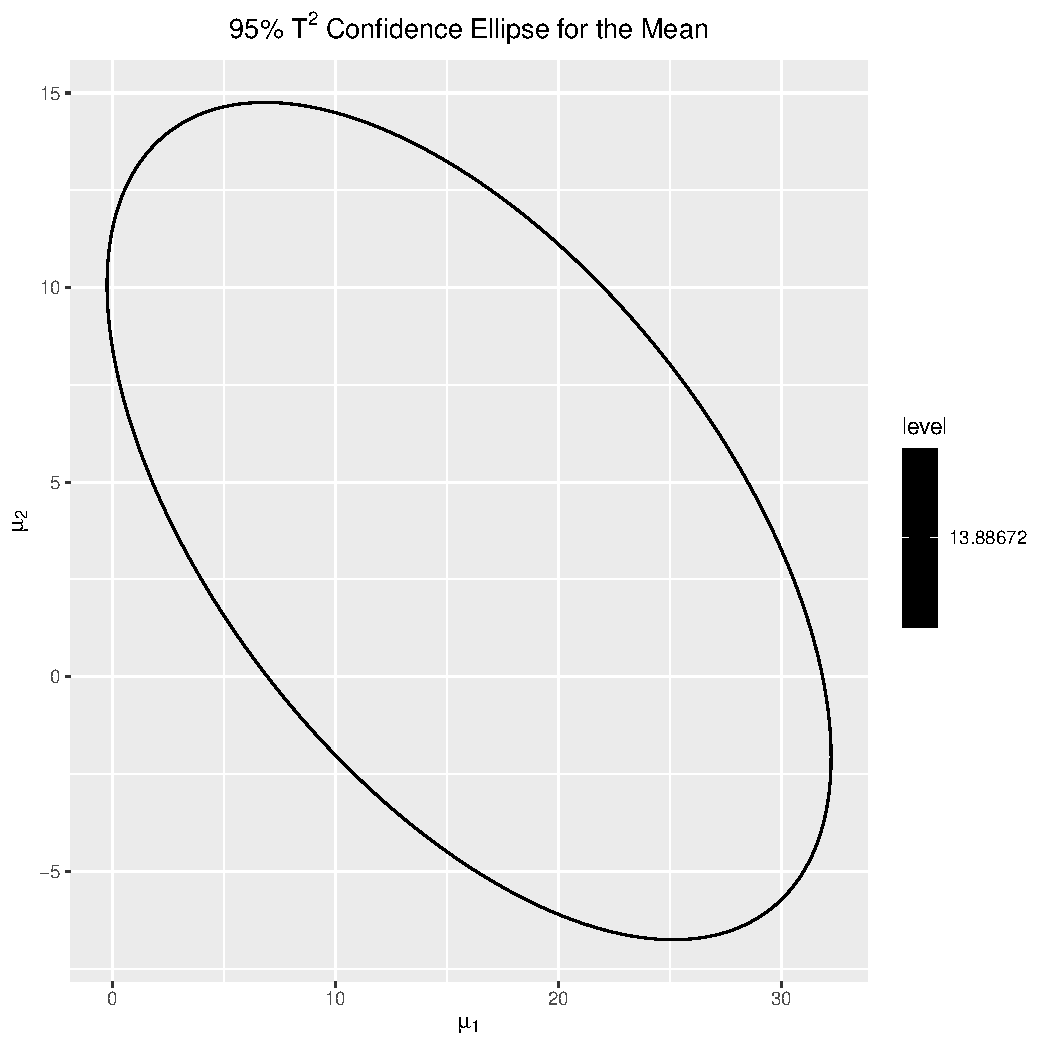
\includegraphics[width=\maxwidth]{figure/unnamed-chunk-2-1} 

\end{knitrout}


%%%%%%%%%%%%%%%%%%%%%%%%%%%%%%%%%%%%%%%%%%%%%%%%%%%%%%%%%%%%%%%%%%%%%%%%%%%%%%%%%%%%%%%%%%%%%%%%%%%%%%%%%%%%%%%%%%%%%%%%%%%%%%%%%%%%%
\newpage
\begin{problem}{5.11(a)}
\end{problem}

We have,
\begin{align*}
\vct{\overline{x}} = \begin{bmatrix} 5.185556 \\ 16.070000 \end{bmatrix}
\end{align*}

and,
\begin{align*}
\vct{S} = \begin{bmatrix} 176.0042 & 287.2412 \\ 287.2412 & 527.8493 \end{bmatrix}
\end{align*}

which implies,
\begin{align*}
\vct{S}^{-1} = \begin{bmatrix} 0.05077341 & -0.02762951 \\ -0.02762951 & 0.01692971 \end{bmatrix}
\end{align*}

Thus, 
\begin{align*}
T^2 &= n(\vct{\overline{x}} - \vct{\mu})' S^{-1} (\vct{\overline{x}} - \vct{\mu})\\
&= 9 \begin{bmatrix} 5.185556 - \mu_1 & 16.070000 - \mu_2 \end{bmatrix} \begin{bmatrix} 0.05077341 & -0.02762951 \\ -0.02762951 & 0.01692971 \end{bmatrix} \begin{bmatrix} 5.185556 - \mu_1 \\ 16.070000 - \mu_2 \end{bmatrix}\\
&= 0.456961 (\mu_1^2 - 1.08835(\mu_1)(\mu_2) + 7.11859\mu_1 + 0.333436 (\mu_2)^2 - 5.07297\mu_2 + 22.3043)
\end{align*}

In addition, the test statistic (with $\alpha = 0.1$) is,
\begin{align*}
\frac{p(n-1)}{(n-p)}F_{p, n-p}(\alpha) &= \frac{2(9-1)}{(9-2)}F_{2, 9-2}(0.1)\\
&= \frac{16}{7}F_{2, 7}(0.1) \approx 7.445582
\end{align*}

Thus, by Example 5.5 in the textbook, the equation for the joint confidence ellipse is,
\begin{align*}
0.456961 (\mu_1^2 - 1.08835(\mu_1)(\mu_2) + 7.11859\mu_1 + 0.333436 (\mu_2)^2 - 5.07297\mu_2 + 22.3043) \leq 7.445582
\end{align*}

which yields the following graph,

\begin{knitrout}
\definecolor{shadecolor}{rgb}{0.969, 0.969, 0.969}\color{fgcolor}
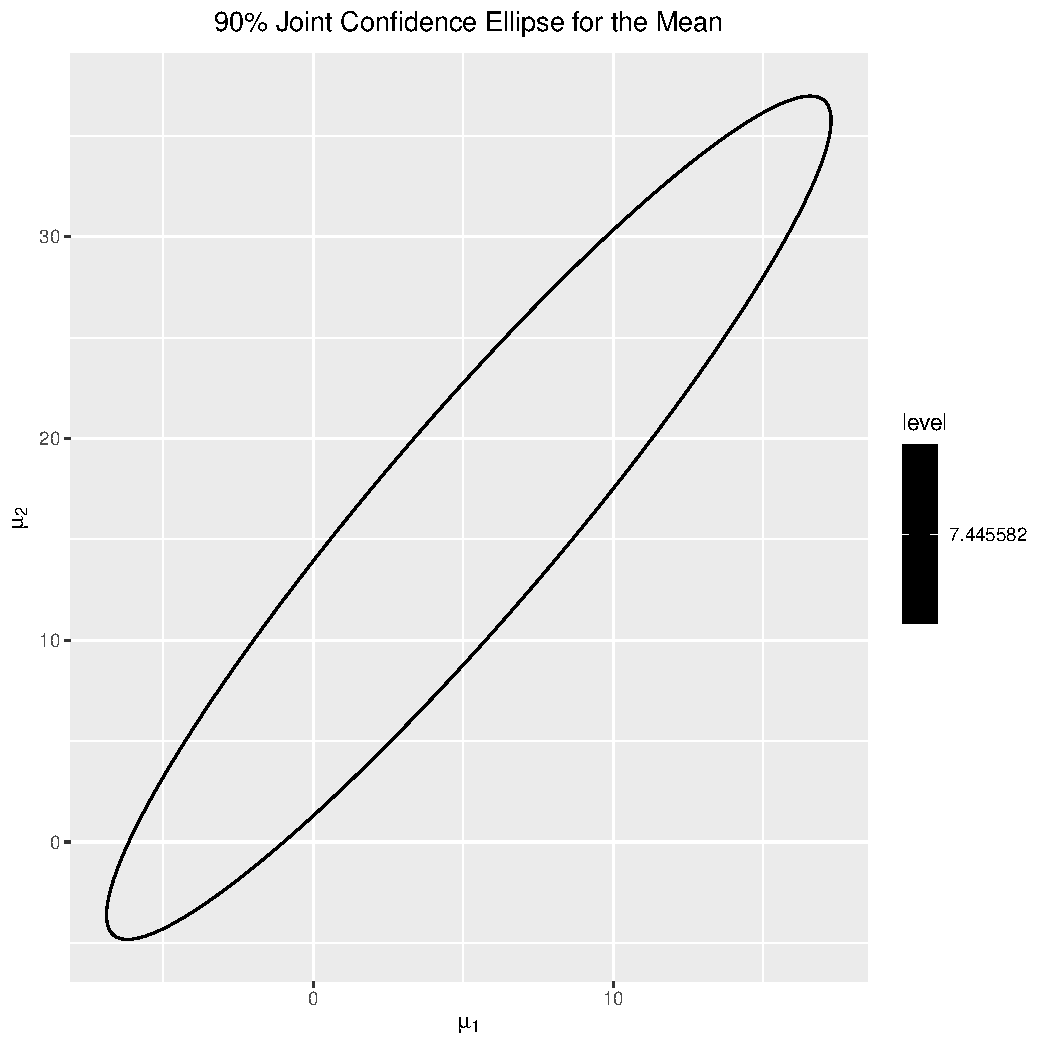
\includegraphics[width=\maxwidth]{figure/unnamed-chunk-3-1} 

\end{knitrout}


%%%%%%%%%%%%%%%%%%%%%%%%%%%%%%%%%%%%%%%%%%%%%%%%%%%%%%%%%%%%%%%%%%%%%%%%%%%%%%%%%%%%%%%%%%%%%%%%%%%%%%%%%%%%%%%%%%%%%%%%%%%%%%%%%%%%%
\newpage
\begin{problem}{5.13}
\end{problem}

We know that $\Lambda^{(2/n)} = \left(\frac{|\hat{\vct{\Sigma}}|}{|\hat{\vct{\Sigma}}_0|}\right)$ with,
\begin{align*}
\Lambda = \frac{\max_{\vct{\Sigma}} L(\vct{\mu}_0, \vct{\Sigma})}{\max_{\vct{\Sigma}, \vct{\mu}} L(\vct{\mu}, \vct{\Sigma})}
\end{align*}

Thus, we have,
\begin{align}
\begin{split}
-n \ln{(|\hat{\vct{\Sigma}}|/|\hat{\vct{\Sigma}}_0|)} &= -n \ln{(\Lambda^{(2/n)})}\\
&= -n (2/n) \ln{\left(\frac{\max_{\vct{\Sigma}} L(\vct{\mu}_0, \vct{\Sigma})}{\max_{\vct{\Sigma}, \vct{\mu}} L(\vct{\mu}, \vct{\Sigma})}\right)}\\
&= -2 \ln{\left(\frac{\max_{\vct{\Sigma}} L(\vct{\mu}_0, \vct{\Sigma})}{\max_{\vct{\Sigma}, \vct{\mu}} L(\vct{\mu}, \vct{\Sigma})}\right)}
\end{split}
\end{align}

We know from the discussion on p. 219 in the textbook that we have $v = p + p(p+1)/2$ and $v_0 = p(p+1)/2$ in this case. Thus, using the data from Table 1, we have $v = 3 + 3(4)/2 = 9$ and $v_0 = 6$. As a result, $v - v_0 = 3$.\\

Hence, from result 5.2 and derivation (1), we have that $n \ln{(|\hat{\vct{\Sigma}}|/|\hat{\vct{\Sigma}}_0|)}$ is distributed approximately as $\chi^2_{3}$.
\end{document}
